% Copyright (c) 2015 Daniele Masini - d.masini.it@gmail.com

\section{Esercizi}
\subsection{Esercizi dei singoli paragrafi}

\begingroup
\hypersetup{linkcolor=black}
\subsubsection*{\ref{sect:metodo_assiomatico_concetti_primitivi} - 
\nameref{sect:metodo_assiomatico_concetti_primitivi}}
\endgroup

\begin{esercizio}
\label{ese:1.15}
Trasforma nella forma <<Se \ldots{} allora \ldots{}>> le seguenti 
frasi:
\begin{enumeratea}
\item <<Un oggetto lanciato verso l'alto ricade a terra>>
\item <<Quando piove prendo l'ombrello>>
\item <<I numeri la cui ultima cifra è 0 sono divisibili per 5>>
\item <<Per essere promosso occorre aver raggiunto la sufficienza>>
\end{enumeratea}
\end{esercizio}


\begin{esercizio}
\label{ese:1.17}
Completa i seguenti ragionamenti:
\begin{enumeratea}
\item <<Se un numero è multiplo di 10 allora è pari>>; <<il numero 
\(n\) non è pari quindi \ldots\ldots\ldots\ldots>>
\item <<Se il sole tramonta fa buio>>; <<il sole è tramontato quindi 
\ldots\ldots\ldots\ldots>>
\end{enumeratea}
\end{esercizio}

\begin{esercizio}
\label{ese:1.18}
Distingui nelle seguenti frasi le definizioni dalle proposizioni o 
proprietà
\begin{enumeratea}
\item <<La Terra ruota su se stessa in un giorno>>		
			\hfill\boxD\quad\boxP
\item <<Il solstizio è il momento in cui il Sole raggiunge, nel suo 
moto apparente lungo l'eclittica, il punto di declinazione massima o 
minima>>			\hfill\boxD\quad\boxP
\item <<La cellula è l'unità fondamentale di tutti gli organismi 
viventi>>\hfill\boxD\quad\boxP
\item <<I virus sono responsabili di alcune 
malattie>>\hfill\boxD\quad\boxP
\item <<I numeri che hanno per ultima cifra 0 sono numeri 
pari>>\hfill\boxD\quad\boxP
\item <<Un numero si dice pari se è divisibile per 
2>>\hfill\boxD\quad\boxP
\end{enumeratea}
\hfill [a)~P,\quad b)~D,\quad c)~D,\quad d)~P,\quad e)~P,\quad f)~D.]
\end{esercizio}

\begin{esercizio}
\label{ese:1.19}
Dimostra con un controesempio che l'affermazione <<Tutti i multipli 
di 3 sono dispari>> non è vera.
\hfill [Un controesempio è 6, che è pari.]
\end{esercizio}


\begin{esercizio}[I Giochi di Archimede, 1997]
\label{ese:1.28}
<<Se il pomeriggio ho giocato a tennis, la sera ho fame e se la sera 
ho fame, allora mangio troppo>>. Quale delle seguenti conclusioni non 
posso trarre da queste premesse?
\begin{enumeratea}
\item <<Se gioco a tennis il pomeriggio, allora la sera ho fame e 
mangio troppo>>;
\item <<Se la sera ho fame, allora mangio troppo, oppure ho giocato a 
tennis il pomeriggio>>;
\item <<Se la sera non ho fame, allora non ho giocato a tennis il 
pomeriggio>>;
\item <<Se la sera non ho fame, allora non mangio troppo>>;
\item <<Se la sera non mangio troppo, allora non ho giocato a tennis 
il pomeriggio>>.
\end{enumeratea}
\end{esercizio}


\begin{esercizio}
\label{ese:1.33}
Gli enti primitivi della geometria sono quelli...
\begin{enumeratea}
\item che occorre definire;
\item che occorre dimostrare;
\item che non si definiscono;
\item che si conoscono già per averli studiati prima.
\end{enumeratea}
\hfill [c]
\end{esercizio}

\begin{esercizio}
\label{ese:1.34}
Gli assiomi sono:
\begin{enumeratea}
\item proposizioni note che si preferisce non dimostrare per non 
appesantire lo studio;
\item proposizioni che è necessario dimostrare;
\item proposizioni che si assumono vere senza dimostrazione;
\item proposizioni che non si definiscono;
\item proposizioni che non si dimostrano perché la loro dimostrazione 
è molto semplice.
\end{enumeratea}
\hfill [c]
\end{esercizio}
	
\begin{esercizio}
\label{ese:1.35}
Quali delle seguenti affermazioni sono vere?
\begin{enumeratea}
\item Due punti sono sempre allineati \hfill \boxV\quad\boxF
\item Tre punti sono sempre allineati \hfill \boxV\quad\boxF
\item Tre punti sono sempre complanari \hfill \boxV\quad\boxF
\item Tre punti allineati individuano un unico piano \hfill \boxV\quad\boxF
\item Una retta e un punto esterno ad essa individuano un piano \hfill 
\boxV\quad\boxF
\end{enumeratea}
\hfill [a)~V,\quad b)~F,\quad c)~V,\quad d)~V,\quad e)~V.]
\end{esercizio}

\begin{esercizio}
\label{ese:1.36}
Su una retta si segnano quattro punti \(A\), \(B\), \(C\) e \(D\). Quanti 
segmenti restano individuati?
\end{esercizio}

\begin{esercizio}
\label{ese:1.37}
Date tre semirette \(a\), \(b\) e \(c\) aventi la stessa origine \(O\), 
quanti angoli restano individuati?
\end{esercizio}

\begin{esercizio}
\label{ese:1.38}
Unisci in tutti i modi possibili, mediante delle rette, tre punti non 
allineati e posti sullo stesso piano.
\end{esercizio}

\begin{esercizio}
\label{ese:1.39}
Unisci in tutti i modi possibili, mediante delle rette, quattro 
punti, a tre a tre non allineati, di uno stesso piano.
\end{esercizio}

\begin{esercizio}
\label{ese:1.40}
Quattro rette a due a due incidenti quanti punti di intersezione 
individuano complessivamente?
\end{esercizio}

\begin{esercizio}
\label{ese:1.41}
Quale assioma è rappresentato nella figura?
\hfill[a]

\begin{minipage}{.59 \textwidth}
\begin{enumeratea}
\item tre punti distinti non allineati determinano uno ed un solo 
piano che li contiene;
\item su un piano esistono infiniti punti ed infinite rette;
\item la retta passante per due punti distinti di un piano giace 
completamente nel piano;
\item su una retta esistono infiniti punti.
\end{enumeratea}
\end{minipage}
\hfil
\begin{minipage}{.39 \textwidth}
\begin{inaccessibleblock}[Piano con disegnati tre punti.]
\centering% Copyright (c) 2015 Daniele Masini - d.masini.it@gmail.com

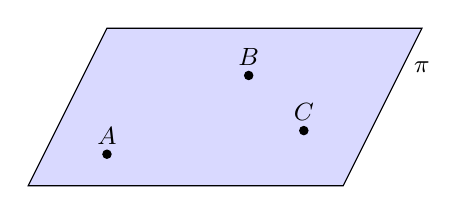
\begin{tikzpicture}[scale=1,font=\small]
\usetikzlibrary{calc}

\begin{scope}
\draw[fill, blue!15] (0,0) -- (1,2) -- (5,2) -- (4,0) -- cycle;
\draw (0,0) -- (1,2) -- (5,2) -- (4,0) -- cycle;
\coordinate (a) at (1,0.4);
\coordinate (b) at (2.8,1.4);
\coordinate (c) at (3.5,.7);
\draw[fill] (a) circle (1.5pt) node[above] {$A$};
\draw[fill] (b) circle (1.5pt) node[above] {$B$};
\draw[fill] (c) circle (1.5pt) node[above] {$C$};
\node at (5,1.5) {$\pi$};

\end{scope}

\end{tikzpicture}

\end{inaccessibleblock}
\end{minipage}
\end{esercizio}


% \begin{inaccessibleblock}[Figura: TODO]
%  \begin{figure}[htb]
%  \centering% Copyright (c) 2015 Daniele Masini - d.masini.it@gmail.com

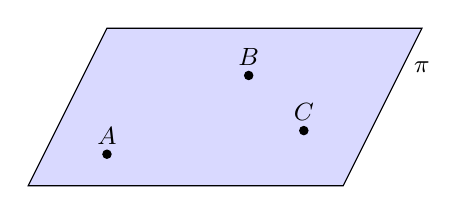
\begin{tikzpicture}[scale=1,font=\small]
\usetikzlibrary{calc}

\begin{scope}
\draw[fill, blue!15] (0,0) -- (1,2) -- (5,2) -- (4,0) -- cycle;
\draw (0,0) -- (1,2) -- (5,2) -- (4,0) -- cycle;
\coordinate (a) at (1,0.4);
\coordinate (b) at (2.8,1.4);
\coordinate (c) at (3.5,.7);
\draw[fill] (a) circle (1.5pt) node[above] {$A$};
\draw[fill] (b) circle (1.5pt) node[above] {$B$};
\draw[fill] (c) circle (1.5pt) node[above] {$C$};
\node at (5,1.5) {$\pi$};

\end{scope}

\end{tikzpicture}

%  \caption{Esercizio \ref{ese:1.41}}\label{fig:ese1.41}
% \end{figure}
% \end{inaccessibleblock}

\begin{esercizio}
\label{ese:1.42}
Rispondi a voce alle seguenti domande
\begin{enumeratea}
\item Qual è l'origine della parola ``geometria''?
\item Qual è la differenza tra ``assioma'' e ``teorema''?
\item Qual è la differenza tra ``ente definito'' e ``ente primitivo''?
\end{enumeratea}
\end{esercizio}

\begingroup
\hypersetup{linkcolor=black}
\subsubsection*{\ref{sect:prime_definizioni} - 
\nameref{sect:prime_definizioni}}
\endgroup

\begin{esercizio}
\label{ese:1.43}
Disegna una retta \(a\) e una retta \(b\) che si incontrano in un punto 
\(X\), disegna anche una retta \(c\) che incontra la \(a\) in \(Y\) e la \(b\) 
in \(Z\). Elenca tutte le semirette e tutti i segmenti che si vengono a 
formare.
\end{esercizio}

\begin{esercizio}
\label{ese:1.44}
Disegna due rette \(a\) e \(b\) parallele tra di loro; disegna poi la 
retta \(c\) che interseca la \(a\) in \(A\) e la \(b\) in \(B\); disegna poi la 
retta \(d\) che interseca \(a\) in \(A\) e \(b\) in \(C\). Quali segmenti si 
vengono a formare?
\end{esercizio}

\begin{esercizio}
\label{ese:1.45}
Rappresenta graficamente ciascuna delle seguenti situazioni:
\begin{enumeratea}
\item \(A\in r\)~~e~~\(B\in r\),~~\(B\in s\)~~e~~\(C\in s\),~~\(A\in 
t\)~~e~~\(C\in t\)
\item \(AB\subset r\),~~\(CD\subset r\),~~\(AB\cap CD=AD\).~~\(AB\cup 
CD=\ldots{}\)
\item \(AB\subset r\),~~\(CD\subset r\),~~\(AB\cap CD=\emptyset\).~~\(AB\cup 
CD=\ldots{}\)
\item \(AB\subset r\),~~\(CD\subset s\),~~\(r\parallel s\),~~\(P\notin r\cup 
s\)
\end{enumeratea}
\end{esercizio}

\begin{esercizio}
\label{ese:1.46}
Attribuisci il nome corretto a ciascuna coppia di segmenti 
rappresentati nella figura~\ref{fig:ese1.46} tra: adiacenti, 
incidenti, disgiunti, consecutivi.
\end{esercizio}


\begin{inaccessibleblock}[Figura: TODO]
 \begin{figure}[htb]
 \centering% Copyright (c) 2015 Daniele Masini - d.masini.it@gmail.com

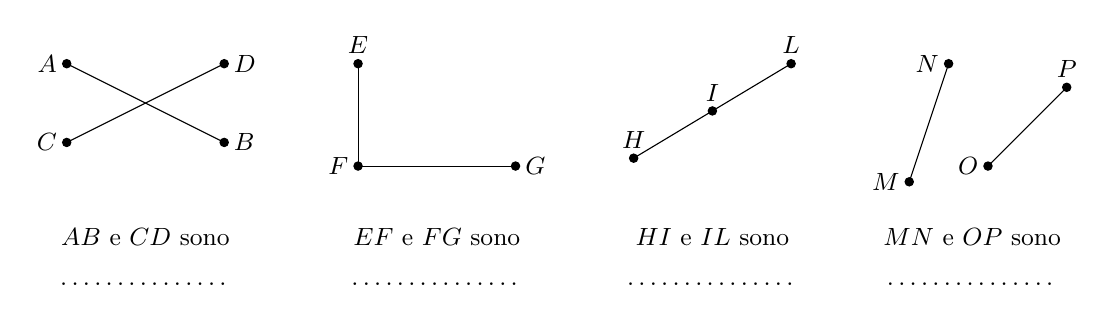
\begin{tikzpicture}[scale=1,font=\small]
\usetikzlibrary{calc}

\begin{scope}
\coordinate (a) at (0,0);
\coordinate (b) at (2,-1);
\coordinate (c) at (0,-1);
\coordinate (d) at (2,0);
\draw (a) node[left] {$A$} -- (b) node[right] {$B$};
\draw (c) node[left] {$C$} -- (d) node[right] {$D$};
\draw[fill] (a) circle (1.5pt) (b) circle (1.5pt) (c) circle (1.5pt) (d) circle (1.5pt);
\node at (1,-2.2) {$AB$ e $CD$ sono};
\node at (1,-2.8) {\ldots\ldots\ldots\ldots\ldots};
\end{scope}

\begin{scope}[xshift=3.7cm]
\coordinate (e) at (0,0);
\coordinate (f) at (0,-1.3);
\coordinate (g) at (2,-1.3);
\draw (e) node[above] {$E$} -- (f) node[left] {$F$} -- (g) node[right] {$G$};
\draw[fill] (e) circle (1.5pt) (f) circle (1.5pt) (g) circle (1.5pt);
\node at (1,-2.2) {$EF$ e $FG$ sono};
\node at (1,-2.8) {\ldots\ldots\ldots\ldots\ldots};
\end{scope}

\begin{scope}[xshift=7.2cm]
\coordinate (h) at (0,-1.2);
\coordinate (i) at (1,-0.6);
\coordinate (l) at (2,0);
\draw (h) node[above] {$H$} -- (i) node[above] {$I$} -- (l) node[above] {$L$};
\draw[fill] (h) circle (1.5pt) (i) circle (1.5pt) (l) circle (1.5pt);
\node at (1,-2.2) {$HI$ e $IL$ sono};
\node at (1,-2.8) {\ldots\ldots\ldots\ldots\ldots};
\end{scope}

\begin{scope}[xshift=10.7cm]
\coordinate (m) at (0,-1.5);
\coordinate (n) at (0.5,0);
\coordinate (o) at (1,-1.3);
\coordinate (p) at (2,-0.3);
\draw (m) node[left] {$M$} -- (n) node[left] {$N$};
\draw (o) node[left] {$O$} -- (p) node[above] {$P$};
\draw[fill] (m) circle (1.5pt) (n) circle (1.5pt) (o) circle (1.5pt) (p) circle (1.5pt);
\node at (0.8,-2.2) {$MN$ e $OP$ sono};
\node at (0.8,-2.8) {\ldots\ldots\ldots\ldots\ldots};
\end{scope}

\end{tikzpicture}

 \caption{Esercizio \ref{ese:1.46}}\label{fig:ese1.46}
\end{figure}
\end{inaccessibleblock}

\begin{esercizio}
\label{ese:1.47}
Su una retta \(r\) disegna i punti \(A\) e \(B\), sapendo che \(A\) precede 
\(B\), disegna i punti \(C\) e \(D\) sapendo che \(D\) è compreso tra \(A\) e 
\(B\) e che \(C\) segue \(B\). Indica tutti i segmenti che si vengono a 
formare.
\end{esercizio}

\begin{esercizio}
\label{ese:1.48}
Dati cinque punti nel piano, in modo che a tre a tre non siano 
allineati, quante rette passanti per due di questi punti è possibile 
tracciare? Sai esprimere il legame generale tra il numero \(N\) di 
punti e il numero \(M\) di rette che si possono tracciare?
\end{esercizio}

\begin{esercizio}
\label{ese:1.49}
Vero o falso?
\vspace{-.5em}
\begin{enumeratea}
\item Per un punto passa una sola retta \hfill\boxV\quad\boxF
\item Per due punti passa una sola retta \hfill\boxV\quad\boxF
\item Per tre punti passano almeno tre rette \hfill\boxV\quad\boxF
\item Due punti distinti del piano individuano sempre un segmento
\hfill\boxV\quad\boxF
\item Due rette distinte del piano hanno al più un punto in comune 
\hfill\boxV\quad\boxF
\item Tre punti distinti del piano individuano almeno tre rette
\hfill\boxV\quad\boxF
\item Due semirette distinte del piano che hanno la stessa origine 
sono opposte \hfill\boxV\quad\boxF
\item Alcuni segmenti consecutivi non sono adiacenti
\hfill\boxV\quad\boxF
\item Due angoli che hanno il vertice in comune sono consecutivi 
\hfill\boxV\quad\boxF
\item Per un punto del piano passano solo due rette
\hfill\boxV\quad\boxF
\item Due segmenti posti sulla stessa retta sono adiacenti
\hfill\boxV\quad\boxF
\item Due segmenti consecutivi hanno in comune un estremo e nessun altro punto 
\hfill\boxV\quad\boxF
\end{enumeratea}
 \hfill[a)~F,\quad b)~V,\quad c)~F,\quad d)~V,\quad e)~V,\quad f)~F,\quad 
g)~F,\quad h)~F,\quad i)~F,\quad j)~F,\quad k)~F,\quad l)~V.]
\end{esercizio}

\begin{esercizio}
\label{ese:1.50}
Due segmenti si dicono adiacenti se:
\begin{enumeratea}
\item appartengono alla stessa retta;
\item sono consecutivi ma non appartengono alla stessa retta;
\item non sono consecutivi e appartengono alla stessa retta;
\item sono consecutivi e appartengono alla stessa retta;
\item appartengono alla stessa retta e hanno gli estremi coincidenti.
\hfill[e]
\end{enumeratea}
\end{esercizio}

\begin{esercizio}
\label{ese:1.51}
Un angolo è convesso se:
\begin{multicols}{2}
\begin{enumeratea}
\item è adiacente ad un altro angolo;
\item i suoi lati sono rette incidenti;
\item contiene il prolungamento dei suoi lati;
\item è consecutivo ad un altro angolo;
\item non contiene il prolungamento \\ 
      dei suoi lati.
\hfill[e]
\end{enumeratea}
\end{multicols}
\end{esercizio}

% \pagebreak

\begin{esercizio}
\label{ese:1.52}
Due angoli si dicono opposti al vertice se:
\begin{multicols}{2}
\begin{enumeratea}
\item sono sullo stesso piano;
\item sono uno concavo e uno convesso;
\item hanno il vertice in comune;
\item i lati dell'uno sono contenuti nell'altro;
\item i lati dell'uno sono il prolungamento \\ 
      dei lati dell'altro.
\hfill[e]
\end{enumeratea}
\end{multicols}
\end{esercizio}

\begin{esercizio}
\label{ese:1.53}
Quanti angoli individuano tre semirette aventi la stessa origine? Fai 
un disegno.
\end{esercizio}

\begin{esercizio}
\label{ese:1.54}
Dà la definizione di ``angolo''.
\end{esercizio}

\begin{esercizio}
\label{ese:1.55}
Qual è la differenza tra angolo piatto e angolo nullo? \emph{Fai 
riferimento alle definizioni e non al fatto che il primo misura 
\(360\grado\) e il secondo \(0\grado\).}
\end{esercizio}

\begin{esercizio}
\label{ese:1.56}
Qual è la differenza tra angoli consecutivi e angoli adiacenti?
\end{esercizio}

\begin{esercizio}
\label{ese:1.57}
Per ciascuna figura scrivi di che angolo si tratta 
(concavo, adiacenti, consecutivi, opposti al vertice).
\end{esercizio}

\begin{inaccessibleblock}[Figura: TODO]
%  \begin{figure}[!h]
 \centering% Copyright (c) 2015 Daniele Masini - d.masini.it@gmail.com

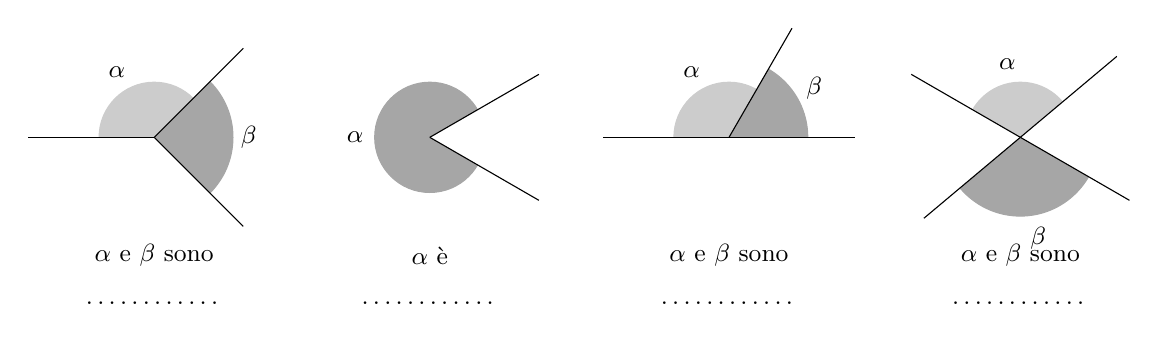
\begin{tikzpicture}
\pgfmathsetmacro{\myscale}{1};

\begin{scope}[scale={\myscale},font=\small]
\usetikzlibrary{calc}

\begin{scope}
\pgfmathsetmacro{\aalpha}{45};
\pgfmathsetmacro{\abeta}{180};
\pgfmathsetmacro{\agamma}{315};

\coordinate (o) at (0,0);
\coordinate (a) at ({\aalpha}:1.6);
\coordinate (b) at ({\abeta}:1.6);
\coordinate (c) at ({\agamma}:1.6);

\begin{scope}
\clip (o) -- (a) -- (-1,1) -- (b) -- cycle;
\draw[gray!40,fill=gray!40] circle[at=(o),radius=.7];
\end{scope}
\node at (120:0.95) {$\alpha$};

\begin{scope}
\clip (o) -- (a) -- (c) -- cycle;
\draw[gray!70,fill=gray!70] circle[at=(o),radius=1];
\end{scope}
\node at (0:1.2) {$\beta$};

\draw (o) -- (a);
\draw (o) -- (b);
\draw (o) -- (c);

\node at (0,-1.5) {$\alpha$ e $\beta$ sono};
\node at (0,-2.1) {\ldots\ldots\ldots\ldots};
\end{scope}

\begin{scope}[xshift=3.5cm]
\pgfmathsetmacro{\aalpha}{30};
\pgfmathsetmacro{\abeta}{330};

\coordinate (o) at (0,0);
\coordinate (a) at ({\aalpha}:1.6);
\coordinate (b) at ({\abeta}:1.6);

\begin{scope}
\clip (o) -- (a) -- (-1,1) -- (-1,-1) -- (b) -- cycle;
\draw[gray!70,fill=gray!70] circle[at=(o),radius=.7];
\end{scope}
\node at (180:0.95) {$\alpha$};

\draw (o) -- (a);
\draw (o) -- (b);

\node at (0,-1.5) {$\alpha$ \`e};
\node at (0,-2.1) {\ldots\ldots\ldots\ldots};
\end{scope}


\begin{scope}[xshift=7.3cm]
\pgfmathsetmacro{\aalpha}{60};
\pgfmathsetmacro{\abeta}{180};
\pgfmathsetmacro{\agamma}{360};

\coordinate (o) at (0,0);
\coordinate (a) at ({\aalpha}:1.6);
\coordinate (b) at ({\abeta}:1.6);
\coordinate (c) at ({\agamma}:1.6);

\begin{scope}
\clip (o) -- (a) -- (b) -- cycle;
\draw[gray!40,fill=gray!40] circle[at=(o),radius=.7];
\end{scope}
\node at (120:0.95) {$\alpha$};

\begin{scope}
\clip (o) -- (a) -- (c) -- cycle;
\draw[gray!70,fill=gray!70] circle[at=(o),radius=1];
\end{scope}
\node at (30:1.25) {$\beta$};

\draw (o) -- (a);
\draw (o) -- (b);
\draw (o) -- (c);

\node at (0,-1.5) {$\alpha$ e $\beta$ sono};
\node at (0,-2.1) {\ldots\ldots\ldots\ldots};
\end{scope}


\begin{scope}[xshift=11cm]
\pgfmathsetmacro{\aalpha}{40};
\pgfmathsetmacro{\abeta}{150};
\pgfmathsetmacro{\agamma}{220};
\pgfmathsetmacro{\adelta}{330};

\coordinate (o) at (0,0);
\coordinate (a) at ({\aalpha}:1.6);
\coordinate (b) at ({\abeta}:1.6);
\coordinate (c) at ({\agamma}:1.6);
\coordinate (d) at ({\adelta}:1.6);

\begin{scope}
\clip (o) -- (a) -- (b) -- cycle;
\draw[gray!40,fill=gray!40] circle[at=(o),radius=.7];
\end{scope}
\node at (100:0.95) {$\alpha$};

\begin{scope}
\clip (o) -- (c) -- (0,-1.3) -- (d) -- cycle;
\draw[gray!70,fill=gray!70] circle[at=(o),radius=1];
\end{scope}
\node at (280:1.3) {$\beta$};

\draw (o) -- (a);
\draw (o) -- (b);
\draw (o) -- (c);
\draw (o) -- (d);

\node at (0,-1.5) {$\alpha$ e $\beta$ sono};
\node at (0,-2.1) {\ldots\ldots\ldots\ldots};
\end{scope}

\end{scope}

\end{tikzpicture}

%  \caption{Esercizio \ref{ese:1.57}}\label{fig:ese1.57}
% \end{figure}
\end{inaccessibleblock}

\newpage %-----------------------------------------------------

\begin{esercizio}
\label{ese:1.58}
Rappresenta graficamente ciascuna delle seguenti situazioni:
\begin{multicols}{2}
% \vspace{-6pt}
\begin{enumeratea}
\item \(A\widehat{O}B\cup A\widehat{O}C=A\widehat{O}B\)
\item \(A\widehat{O}B\cap A\widehat{O}C=A\widehat{O}B\)
\item \(A\widehat{O}B\cap C\widehat{O}D=C\widehat{O}B\)
\item \(A\widehat{O}B\cup C\widehat{O}D=A\widehat{O}B\)
\end{enumeratea}
\end{multicols}
\end{esercizio}

\begin{esercizio}
\label{ese:1.59}
Facendo riferimento alla figura a fianco indica:

\begin{minipage}{.60\textwidth}
\begin{enumeratea}
\item una coppia di segmenti consecutivi \ldots\ldots\ldots\ldots{};
\item una coppia di segmenti adiacenti \ldots\ldots\ldots\ldots{};
\item una coppia di rette incidenti \ldots\ldots\ldots\ldots{};
\item una coppia di rette parallele \ldots\ldots\ldots\ldots{};
\item una coppia di angoli consecutivi \ldots\ldots\ldots\ldots{};
\item una coppia di angoli adiacenti \ldots\ldots\ldots\ldots{};
\item una coppia di angoli opposti al vertice 
\ldots\ldots\ldots\ldots{};
\item un angolo concavo \ldots\ldots\ldots\ldots{};
\item un angolo convesso \ldots\ldots\ldots\ldots{}
\end{enumeratea}
\end{minipage}
\hfill
\begin{minipage}{.34\textwidth}
\begin{inaccessibleblock}[Figura: TODO]
%  \begin{figure}[htb]
 \centering% Copyright (c) 2015 Daniele Masini - d.masini.it@gmail.com

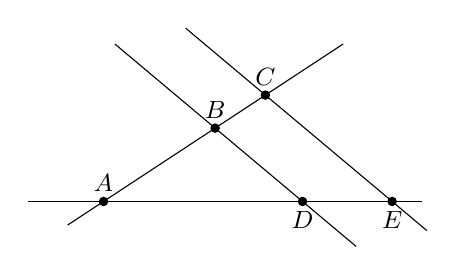
\begin{tikzpicture}[scale=1,font=\small]
\usetikzlibrary{calc}

\begin{scope}
\draw (0,0) coordinate (r1) -- (5,0) coordinate (r2);
\draw  (0.5,-.3) coordinate (s1) -- (4,2) coordinate (s2);
\draw  (1.1,2) coordinate (t1) -- +(-40:4) coordinate (t2);
\draw  (2,2.2) coordinate (u1) -- +(-40:4) coordinate (u2);
\coordinate (a) at (intersection of r1--r2 and s1--s2);
\coordinate (b) at (intersection of t1--t2 and s1--s2);
\coordinate (c) at (intersection of u1--u2 and s1--s2);
\coordinate (d) at (intersection of t1--t2 and r1--r2);
\coordinate (e) at (intersection of u1--u2 and r1--r2);
\draw[fill] (a) circle (1.5pt) node[above] {$A$};
\draw[fill] (b) circle (1.5pt) node[above] {$B$};
\draw[fill] (c) circle (1.5pt) node[above] {$C$};
\draw[fill] (d) circle (1.5pt) node[below] {$D$};
\draw[fill] (e) circle (1.5pt) node[below] {$E$};

\end{scope}


\end{tikzpicture}

%  \caption{Esercizio \ref{ese:1.59}}\label{fig:ese1.59}
% \end{figure}
\end{inaccessibleblock}
\end{minipage}
\end{esercizio}

% \begin{esercizio}
% \label{ese:1.60}
% Indica quali delle figure geometriche riportate nella 
% figura~\ref{fig:ese1.60} sono convesse
% \begin{multicols}{5}
% \begin{enumeratea}
% \item \(A\), \(B\), \(C\), \(G\);
% \item \(B\), \(C\), \(D\), \(F\);
% \item \(B\), \(C\), \(D\);
% \item \(B\), \(C\);
% \item \(D\), \(E\), \(F\), \(G\).
% \end{enumeratea}
% \end{multicols}
% \hfill[c]
% \end{esercizio}
% 
% \begin{inaccessibleblock}[Figura: TODO]
%  \begin{figure}[htb]
%  \centering% Copyright (c) 2015 Daniele Masini - d.masini.it@gmail.com

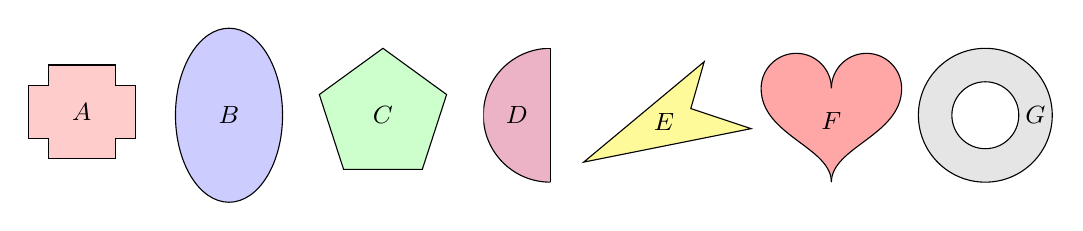
\begin{tikzpicture}[scale=0.85,font=\small]
\usetikzlibrary{calc}

\begin{scope}[yshift=.75cm]
\draw[fill=pink!80] (0,0) -- (1,0) -- (1,-.3) -- (1.3,-.3) -- (1.3,-1.1) -- (1,-1.1) -- (1,-1.4) -- (0,-1.4) -- (0,-1.1) -- (-.3,-1.1) -- (-.3,-.3) -- (0,-.3) -- cycle;
\node at (.5,-.7) {$A$};
\end{scope}

\begin{scope}[xshift=2.7cm]
\draw[fill=blue!20] (0,0) circle [x radius=.8cm, y radius=1.3cm];
\node at (0,0) {$B$};
\end{scope}

\begin{scope}[xshift=5cm,rotate=18]
\coordinate (o) at (0,0);
\coordinate (p0) at (0:1cm);
\coordinate (p1) at (1*72:1cm);
\coordinate (p2) at (2*72:1cm);
\coordinate (p3) at (3*72:1cm);
\coordinate (p4) at (4*72:1cm);
\draw[fill=green!20] (p0) -- (p1) -- (p2) -- (p3) -- (p4) -- cycle;
\node at (o) {$C$};
\end{scope}

\begin{scope}[xshift=7.5cm]
\begin{scope}
\clip (-1,-1.1) rectangle (0,1);
\draw[fill=purple!30] (0,0) circle (1cm);
\end{scope}
\draw (0,-1) -- (0,1);
\node at (-0.5,0) {$D$};
\end{scope}

\begin{scope}[xshift=8cm,yshift=-0.7cm]
\draw[fill=yellow!40] (0,0) -- (2.5,0.5) -- (1.6,0.8) -- (1.8,1.5) -- cycle;
\node at (1.2,0.6) {$E$};
\end{scope}

\begin{scope}[xshift=11.7cm,yshift=-1cm,scale=.7]
\draw[fill=red!35] (0,0) .. controls (0,0.75) and (-1.5,1) .. (-1.5,2)  arc (180:0:0.75);
\draw[red!35] (0,0) -- (0,2);
\draw[fill=red!35] (0,0) .. controls (0,0.75) and ( 1.5,1) .. ( 1.5,2)  arc (0:180:0.75);
\node at (0,1.3) {$F$};
\end{scope}

\begin{scope}[xshift=14cm]
\draw[fill=gray!20] (0,0) circle (1cm);
\begin{scope}
\clip (0,0) circle (1cm);
\draw[fill,white] (0,0) circle (.5cm);
\end{scope}
\draw (0,0) circle (.5cm);
\node at (0.75,0) {$G$};
\end{scope}

\end{tikzpicture}

%  \caption{Esercizio~\ref{ese:1.60}}\label{fig:ese1.60}
% \end{figure}
% \end{ina

\begin{esercizio}
\label{ese:1.60}
Indica quali delle seguenti figure geometriche sono convesse:

\begin{inaccessibleblock}[Figura: Figure concave e convesse]
%  \begin{figure}[!h]
 \centering% Copyright (c) 2015 Daniele Masini - d.masini.it@gmail.com

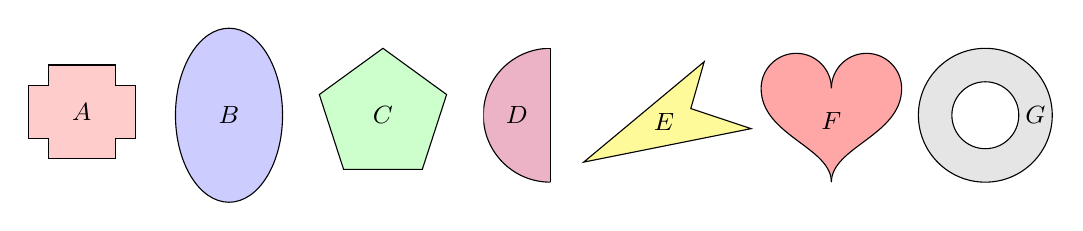
\begin{tikzpicture}[scale=0.85,font=\small]
\usetikzlibrary{calc}

\begin{scope}[yshift=.75cm]
\draw[fill=pink!80] (0,0) -- (1,0) -- (1,-.3) -- (1.3,-.3) -- (1.3,-1.1) -- (1,-1.1) -- (1,-1.4) -- (0,-1.4) -- (0,-1.1) -- (-.3,-1.1) -- (-.3,-.3) -- (0,-.3) -- cycle;
\node at (.5,-.7) {$A$};
\end{scope}

\begin{scope}[xshift=2.7cm]
\draw[fill=blue!20] (0,0) circle [x radius=.8cm, y radius=1.3cm];
\node at (0,0) {$B$};
\end{scope}

\begin{scope}[xshift=5cm,rotate=18]
\coordinate (o) at (0,0);
\coordinate (p0) at (0:1cm);
\coordinate (p1) at (1*72:1cm);
\coordinate (p2) at (2*72:1cm);
\coordinate (p3) at (3*72:1cm);
\coordinate (p4) at (4*72:1cm);
\draw[fill=green!20] (p0) -- (p1) -- (p2) -- (p3) -- (p4) -- cycle;
\node at (o) {$C$};
\end{scope}

\begin{scope}[xshift=7.5cm]
\begin{scope}
\clip (-1,-1.1) rectangle (0,1);
\draw[fill=purple!30] (0,0) circle (1cm);
\end{scope}
\draw (0,-1) -- (0,1);
\node at (-0.5,0) {$D$};
\end{scope}

\begin{scope}[xshift=8cm,yshift=-0.7cm]
\draw[fill=yellow!40] (0,0) -- (2.5,0.5) -- (1.6,0.8) -- (1.8,1.5) -- cycle;
\node at (1.2,0.6) {$E$};
\end{scope}

\begin{scope}[xshift=11.7cm,yshift=-1cm,scale=.7]
\draw[fill=red!35] (0,0) .. controls (0,0.75) and (-1.5,1) .. (-1.5,2)  arc (180:0:0.75);
\draw[red!35] (0,0) -- (0,2);
\draw[fill=red!35] (0,0) .. controls (0,0.75) and ( 1.5,1) .. ( 1.5,2)  arc (0:180:0.75);
\node at (0,1.3) {$F$};
\end{scope}

\begin{scope}[xshift=14cm]
\draw[fill=gray!20] (0,0) circle (1cm);
\begin{scope}
\clip (0,0) circle (1cm);
\draw[fill,white] (0,0) circle (.5cm);
\end{scope}
\draw (0,0) circle (.5cm);
\node at (0.75,0) {$G$};
\end{scope}

\end{tikzpicture}

%  \caption{Figure concave e convesse}\label{fig:ese1.60}
% \end{figure}
\end{inaccessibleblock}
\end{esercizio}

% \vspace{-12pt}
\begin{multicols}{2}

\begin{esercizio}
\label{ese:1.61}
Scrivi per esteso nel linguaggio comune quanto è indicato in simboli 
e rappresenta con un disegno tutti i casi possibili: \((A\in r)\wedge 
(A\in s)\wedge (B\in r)\).
\end{esercizio}

\begin{esercizio}
\label{ese:1.59}
Riproduci nel quaderno e descrivi la costruzione della figura a fianco, 
dove 
le rette \(c\) e \(d\) sono parallele.
\end{esercizio}

\begin{inaccessibleblock}[Figura: Due rette parallele tagliate da due 
trasversali che si intersecano in un punto P]
 \begin{center}
  % Copyright (c) 2015 Daniele Masini - d.masini.it@gmail.com

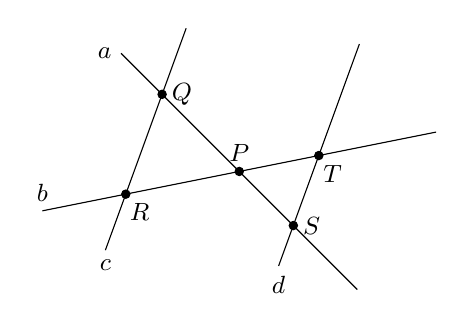
\begin{tikzpicture}[scale=1,font=\small]
\usetikzlibrary{calc}

\begin{scope}
\draw (0,0) node[above] {$b$} coordinate (b1) -- (5,1) coordinate (b2);
\draw (1,2) node[left] {$a$} coordinate (a1) -- (4,-1) coordinate (a2);
\draw (0.8,-0.5) node[below] {$c$} coordinate (c1) -- +(70:3) coordinate (c2);
\draw (3,-0.7) node[below] {$d$} coordinate (d1) -- +(70:3) coordinate (d2);

\coordinate (p) at (intersection of b1--b2 and a1--a2);
\draw[fill] (p) circle (1.5pt) node[above] {$P$}; 
\coordinate (q) at (intersection of a1--a2 and c1--c2);
\draw[fill] (q) circle (1.5pt) node[right] {$Q$}; 
\coordinate (r) at (intersection of b1--b2 and c1--c2);
\draw[fill] (r) circle (1.5pt) node[right=5pt, below] {$R$}; 
\coordinate (s) at (intersection of a1--a2 and d1--d2);
\draw[fill] (s) circle (1.5pt) node[right] {$S$}; 
\coordinate (t) at (intersection of b1--b2 and d1--d2);
\draw[fill] (t) circle (1.5pt) node[right=5pt, below] {$T$}; 

\end{scope}

\end{tikzpicture}

 \end{center}
%  \begin{figure}[!h]
%  \centering% Copyright (c) 2015 Daniele Masini - d.masini.it@gmail.com

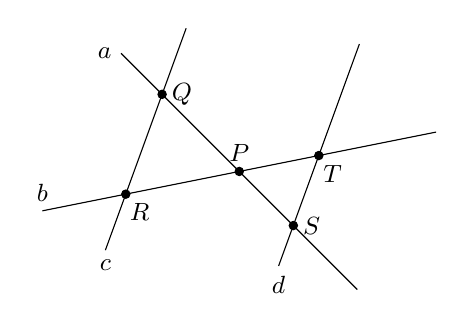
\begin{tikzpicture}[scale=1,font=\small]
\usetikzlibrary{calc}

\begin{scope}
\draw (0,0) node[above] {$b$} coordinate (b1) -- (5,1) coordinate (b2);
\draw (1,2) node[left] {$a$} coordinate (a1) -- (4,-1) coordinate (a2);
\draw (0.8,-0.5) node[below] {$c$} coordinate (c1) -- +(70:3) coordinate (c2);
\draw (3,-0.7) node[below] {$d$} coordinate (d1) -- +(70:3) coordinate (d2);

\coordinate (p) at (intersection of b1--b2 and a1--a2);
\draw[fill] (p) circle (1.5pt) node[above] {$P$}; 
\coordinate (q) at (intersection of a1--a2 and c1--c2);
\draw[fill] (q) circle (1.5pt) node[right] {$Q$}; 
\coordinate (r) at (intersection of b1--b2 and c1--c2);
\draw[fill] (r) circle (1.5pt) node[right=5pt, below] {$R$}; 
\coordinate (s) at (intersection of a1--a2 and d1--d2);
\draw[fill] (s) circle (1.5pt) node[right] {$S$}; 
\coordinate (t) at (intersection of b1--b2 and d1--d2);
\draw[fill] (t) circle (1.5pt) node[right=5pt, below] {$T$}; 

\end{scope}

\end{tikzpicture}

%  \caption{Esercizio~\ref{ese:1.62}}\label{fig:ese1.62}
% \end{figure}
\end{inaccessibleblock}

\end{multicols}

\begin{esercizio}
\label{ese:1.63}
Se \(P\) è centro di un fascio di rette e \(A\) è un punto dello stesso 
piano, è vero che nel fascio di centro \(P\) esiste una retta passante 
per \(A\)?
\hfill[Sì]
\end{esercizio}

\begin{esercizio}
\label{ese:1.64}
Motiva la verità o la falsità della proposizione: <<Tutte le rette 
incidenti formano 2 coppie di angoli opposti al vertice>>.
\end{esercizio}

\begin{esercizio}
\label{ese:1.65}
Siano \(a\), \(b\), \(c\), \(d\) quattro semirette aventi l'origine in comune 
\(O\) disposte in ordine antiorario come nella figura seguente. 
Individua, aiutandoti con il disegno, quali 
sono gli angoli che si ottengono dalle seguenti operazioni:
\noindent \begin{multicols}{5}
\noindent \begin{enumeratea}
\item \(\widehat{ad} \cap \widehat{bd}\)
 % Copyright (c) 2015 Daniele Masini - d.masini.it@gmail.com

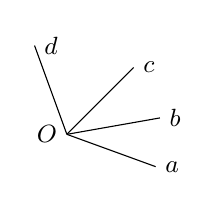
\begin{tikzpicture}[scale=.6,font=\small]
\usetikzlibrary{calc}

\begin{scope}
\pgfmathsetmacro{\aalpha}{-20};
\pgfmathsetmacro{\abeta}{10};
\pgfmathsetmacro{\agamma}{45};
\pgfmathsetmacro{\adelta}{110};

\draw (0,0) coordinate (o) node[left] {$O$} -- +({\aalpha}:2) node[right] {$a$};
\draw (o) -- +({\abeta}:2) node[right] {$b$};
\draw (o) -- +({\agamma}:2) node[right] {$c$};
\draw (o) -- +({\adelta}:2) node[right] {$d$};
\end{scope}

\end{tikzpicture}

\item \(\widehat{cd} \cup \widehat{bc}\)
 % Copyright (c) 2015 Daniele Masini - d.masini.it@gmail.com

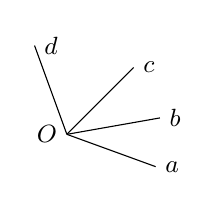
\begin{tikzpicture}[scale=.6,font=\small]
\usetikzlibrary{calc}

\begin{scope}
\pgfmathsetmacro{\aalpha}{-20};
\pgfmathsetmacro{\abeta}{10};
\pgfmathsetmacro{\agamma}{45};
\pgfmathsetmacro{\adelta}{110};

\draw (0,0) coordinate (o) node[left] {$O$} -- +({\aalpha}:2) node[right] {$a$};
\draw (o) -- +({\abeta}:2) node[right] {$b$};
\draw (o) -- +({\agamma}:2) node[right] {$c$};
\draw (o) -- +({\adelta}:2) node[right] {$d$};
\end{scope}

\end{tikzpicture}

\item \(\widehat{cb} \cup \widehat{ac}\)
 % Copyright (c) 2015 Daniele Masini - d.masini.it@gmail.com

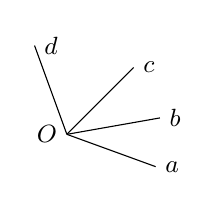
\begin{tikzpicture}[scale=.6,font=\small]
\usetikzlibrary{calc}

\begin{scope}
\pgfmathsetmacro{\aalpha}{-20};
\pgfmathsetmacro{\abeta}{10};
\pgfmathsetmacro{\agamma}{45};
\pgfmathsetmacro{\adelta}{110};

\draw (0,0) coordinate (o) node[left] {$O$} -- +({\aalpha}:2) node[right] {$a$};
\draw (o) -- +({\abeta}:2) node[right] {$b$};
\draw (o) -- +({\agamma}:2) node[right] {$c$};
\draw (o) -- +({\adelta}:2) node[right] {$d$};
\end{scope}

\end{tikzpicture}

\item \(\widehat{ab} \cap \widehat{bd}\)
 % Copyright (c) 2015 Daniele Masini - d.masini.it@gmail.com

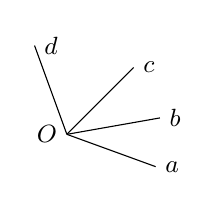
\begin{tikzpicture}[scale=.6,font=\small]
\usetikzlibrary{calc}

\begin{scope}
\pgfmathsetmacro{\aalpha}{-20};
\pgfmathsetmacro{\abeta}{10};
\pgfmathsetmacro{\agamma}{45};
\pgfmathsetmacro{\adelta}{110};

\draw (0,0) coordinate (o) node[left] {$O$} -- +({\aalpha}:2) node[right] {$a$};
\draw (o) -- +({\abeta}:2) node[right] {$b$};
\draw (o) -- +({\agamma}:2) node[right] {$c$};
\draw (o) -- +({\adelta}:2) node[right] {$d$};
\end{scope}

\end{tikzpicture}

\item \(\widehat{ac} \cap \widehat{bd}\)
 % Copyright (c) 2015 Daniele Masini - d.masini.it@gmail.com

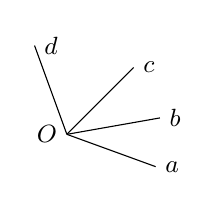
\begin{tikzpicture}[scale=.6,font=\small]
\usetikzlibrary{calc}

\begin{scope}
\pgfmathsetmacro{\aalpha}{-20};
\pgfmathsetmacro{\abeta}{10};
\pgfmathsetmacro{\agamma}{45};
\pgfmathsetmacro{\adelta}{110};

\draw (0,0) coordinate (o) node[left] {$O$} -- +({\aalpha}:2) node[right] {$a$};
\draw (o) -- +({\abeta}:2) node[right] {$b$};
\draw (o) -- +({\agamma}:2) node[right] {$c$};
\draw (o) -- +({\adelta}:2) node[right] {$d$};
\end{scope}

\end{tikzpicture}

\end{enumeratea}
% \begin{enumeratea}
% \item \(a\widehat{O}d \cap d\widehat{O}b\);
% \item \(d\widehat{O}c \cup c\widehat{O}b\);
% \item \(c\widehat{O}b \cup c\widehat{O}a\);
% \item \(a\widehat{O}b \cap d\widehat{O}b\);
% \item \(c\widehat{O}a \cap d\widehat{O}b\).
% \end{enumeratea}
\end{multicols}
\end{esercizio}


% \begin{inaccessibleblock}[Figura: TODO]
%  \begin{figure}[htb]
%  \centering% Copyright (c) 2015 Daniele Masini - d.masini.it@gmail.com

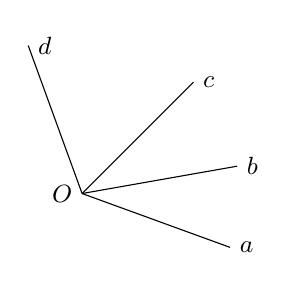
\begin{tikzpicture}[scale=1,font=\small]
\usetikzlibrary{calc}

\begin{scope}
\pgfmathsetmacro{\aalpha}{-20};
\pgfmathsetmacro{\abeta}{10};
\pgfmathsetmacro{\agamma}{45};
\pgfmathsetmacro{\adelta}{110};

\draw (0,0) coordinate (o) node[left] {$O$} -- +({\aalpha}:2) node[right] {$a$};
\draw (o) -- +({\abeta}:2) node[right] {$b$};
\draw (o) -- +({\agamma}:2) node[right] {$c$};
\draw (o) -- +({\adelta}:2) node[right] {$d$};
\end{scope}

\end{tikzpicture}

%  \caption{Esercizio~\ref{ese:1.65}}\label{fig:ese1.65}
% \end{figure}
% \end{inaccessibleblock}

\begingroup
\hypersetup{linkcolor=black}
\subsubsection*{\ref{sect:operazioni_segmenti_angoli} - 
\nameref{sect:operazioni_segmenti_angoli}}
\endgroup

\begin{esercizio}
\label{ese:1.66}
Due angoli sono complementari e uno è doppio dell'altro. Quale delle 
seguenti affermazioni è vera?
\vspace{-.5em}
\begin{enumeratea}
\item uno è retto e l'altro è piatto;
\item uno è \(1/3\) dell'angolo retto e l'altro i \(2/3\) dell'angolo 
retto;
\item uno è \(1/3\) dell'angolo retto e l'altro \(1/6\) dell'angolo retto;
\item uno è \(1/2\) dell'angolo retto e l'altro è retto;
\item uno è \(2/3\) dell'angolo retto e l'altro i \(4/6\) dell'angolo 
retto.
\end{enumeratea}
\end{esercizio}

\begin{esercizio}
\label{ese:1.67}
Siano \(\alpha\) e \(\beta\) due angoli consecutivi esplementari e siano 
\(a\) e \(b\) le loro bisettrici. L'angolo tra \(a\) e \(b\) è
\vspace{-.5em}
\begin{multicols}{3}
\begin{enumeratea}
\item nullo;
\item acuto;
\item retto;
\item piatto;
\item non si può sapere.
\end{enumeratea}
\end{multicols}
\vspace{-18pt}
\hfill[a]
\end{esercizio}

\begin{esercizio}
\label{ese:1.68}
Se \(\alpha\) e \(\beta\) sono due angoli di vertice \(O\), consecutivi e 
complementari e \(a\) e \(b\) le loro bisettrici, allora dell'angolo 
\(a\widehat{O}b\) si può dire  che:
\vspace{-.5em}
\begin{multicols}{2}
\begin{enumeratea}
\item è uguale all'angolo retto;
\item è la metà di un angolo retto;
\item è la terza parte di un angolo retto;
\item è la quarta parte di un angolo retto;
\item non si può determinarne l'ampiezza.
\end{enumeratea}
\end{multicols}
\vspace{-18pt}
\hfill[b]
\end{esercizio}

\begin{esercizio}
\label{ese:1.69}
Le bisettrici di due angoli adiacenti:
\vspace{-.5em}
\begin{multicols}{2}
\begin{enumeratea}
\item sono parallele;
\item sono lati di un angolo retto;
\item sono lati di un angolo concavo;
\item coincidono;
\item sono semirette opposte.
\end{enumeratea}
\end{multicols}
\vspace{-18pt}
\hfill[b]
\end{esercizio}

\begin{esercizio}
\label{ese:1.70}
Due angoli si dicono complementari quando:
\vspace{-.5em}
\begin{multicols}{2}
\begin{enumeratea}
\item sono consecutivi;
\item sono angoli opposti al vertice;
\item la loro somma è un angolo retto;
\item ciascuno di essi è acuto;
\item ciascuno è la metà di un angolo retto.
\end{enumeratea}
\end{multicols}
\vspace{-18pt}
\hfill[c]
\end{esercizio}

\begin{esercizio}
\label{ese:1.71}
Dati due segmenti adiacenti \(AB\) e \(BC\) tali che \(AB\cong 
\frac{1}{3}\cdot BC\), allora per \(AC=AB+BC\) si può dire che:
\vspace{-.5em}
\begin{multicols}{3}
\begin{enumeratea}
\item \(AC\cong \frac{1}{4}\cdot BC\);
\item \(AC\cong 3\cdot BC\);
\item \(AC\cong 2\cdot BC\);
\item \(AC\cong \frac{1}{2}\cdot BC\);
\item \(AC\cong \frac{4}{3}\cdot BC\).
\end{enumeratea}
\end{multicols}
\vspace{-18pt}
\hfill[e]
\end{esercizio}

\begin{esercizio}
\label{ese:1.72}
Due segmenti \(AB\) e \(CD\) appartengono alla stessa retta e hanno lo 
stesso punto medio. Si può affermare che:
\vspace{-.5em}
\begin{multicols}{5}
\begin{enumeratea}
\item \(AB\cong CD\);
\item \(AC\cong CD\);
\item \(DB\cong DC\);
\item \(AC\cong BD\);
\item \(AC\cong AB\).
\end{enumeratea}
\end{multicols}
\vspace{-18pt}
\hfill[d]
\end{esercizio}

\begin{esercizio}
\label{ese:1.73}
Per ciascuna delle affermazioni seguenti, dire se è vera o falsa, e 
spiegare perché
\begin{enumeratea}
\item l'angolo retto è la metà dell'angolo giro
\hfill \boxV\quad\boxF
\item ogni angolo convesso ha due bisettrici
\hfill \boxV\quad\boxF
\item due angoli che hanno in comune il vertice sono consecutivi
\hfill \boxV\quad\boxF
\item un angolo ottuso è maggiore di qualunque angolo acuto
\hfill \boxV\quad\boxF
\item sommando due angoli acuti si può ottenere un angolo piatto
\hfill \boxV\quad\boxF
\end{enumeratea}
\vspace{-.5em}
\hfill[a)~F,\quad b)~F,\quad c)~F,\quad d)~V,\quad e)~F.]
\end{esercizio}

\begin{esercizio}
\label{ese:1.74}
Tre semirette \(a\), \(b\), \(c\) uscenti da uno stesso punto dividono il 
piano in tre angoli congruenti. Dopo aver rappresentato le semirette, 
traccia la semiretta \(b_1\) opposta di \(b\). Quale delle seguenti 
affermazioni è vera?
\begin{enumeratea}
\item \(b_1\) è perpendicolare alla semiretta \(a\);
\item \(b_1\) è bisettrice dell'angolo formato da \(a\) e \(c\);
\item \(b_1\) è perpendicolare alla semiretta \(c\);
\end{enumeratea}
\vspace{-18pt}
\hfill[b]
\end{esercizio}

\begin{multicols}{2}
\begin{esercizio}
\label{ese:1.75}
Dato l'angolo acuto \(A\widehat{O}B\), sia \(OC\) la sua bisettrice. Sia 
poi \(OD\) una semiretta esterna all'angolo quale relazione è vera?
% \begin{multicols}{2}
\begin{enumeratea}
\item \(C\widehat{O}B\cong 
\frac{1}{2}\cdot(D\widehat{O}A-D\widehat{O}B)\)
\item \(C\widehat{O}B\cong (A\widehat{O}D-A\widehat{O}B)\)
\item \(C\widehat{O}B\cong (B\widehat{O}D-C\widehat{O}B)\)
\item \(C\widehat{O}B\cong 
\frac{1}{2}\cdot(D\widehat{O}A+D\widehat{O}B)\)\hfill[a]
\end{enumeratea}
% \end{multicols}
% \vspace{-18pt}
% \hfill[a]
\end{esercizio}
\begin{inaccessibleblock}[Figura: TODO]
\begin{center}
 % Copyright (c) 2015 Daniele Masini - d.masini.it@gmail.com

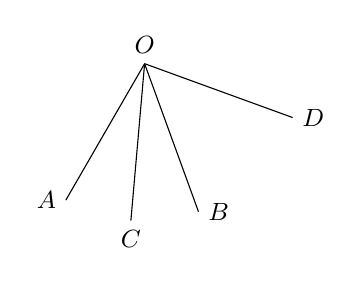
\begin{tikzpicture}[scale=1,font=\small]
\usetikzlibrary{calc}

\begin{scope}
\pgfmathsetmacro{\aalpha}{240};
\pgfmathsetmacro{\abeta}{290};
\pgfmathsetmacro{\agamma}{265};
\pgfmathsetmacro{\adelta}{340};

\draw (0,0) coordinate (o) node[above] {$O$} -- +({\aalpha}:2) node[left] {$A$};
\draw (o) -- +({\abeta}:2) node[right] {$B$};
\draw (o) -- +({\agamma}:2) node[below] {$C$};
\draw (o) -- +({\adelta}:2) node[right] {$D$};
\end{scope}

\end{tikzpicture}

\end{center}
\end{inaccessibleblock}


% \begin{inaccessibleblock}[Figura: TODO]
% %  \begin{figure}[htb]
%  \centering% Copyright (c) 2015 Daniele Masini - d.masini.it@gmail.com

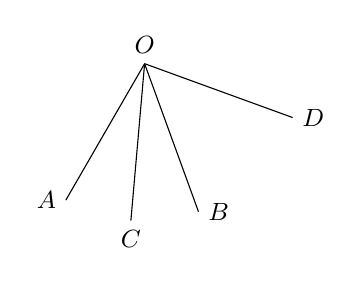
\begin{tikzpicture}[scale=1,font=\small]
\usetikzlibrary{calc}

\begin{scope}
\pgfmathsetmacro{\aalpha}{240};
\pgfmathsetmacro{\abeta}{290};
\pgfmathsetmacro{\agamma}{265};
\pgfmathsetmacro{\adelta}{340};

\draw (0,0) coordinate (o) node[above] {$O$} -- +({\aalpha}:2) node[left] {$A$};
\draw (o) -- +({\abeta}:2) node[right] {$B$};
\draw (o) -- +({\agamma}:2) node[below] {$C$};
\draw (o) -- +({\adelta}:2) node[right] {$D$};
\end{scope}

\end{tikzpicture}

% %  \caption{Esercizio~\ref{ese:1.75}}\label{fig:ese1.75}
% % \end{figure}
% \end{inaccessibleblock}
\end{multicols}

\begin{esercizio}
\label{ese:1.76}
Individua tra gli angoli rappresentati nella figura 
quello piatto, quello retto, quello acuto, quello ottuso e quello 
concavo, scrivendolo nelle relative etichette. 
Per ciascuno di essi traccia la bisettrice.
\begin{center}
\begin{inaccessibleblock}[Figura: TODO]
 % Copyright (c) 2015 Daniele Masini - d.masini.it@gmail.com

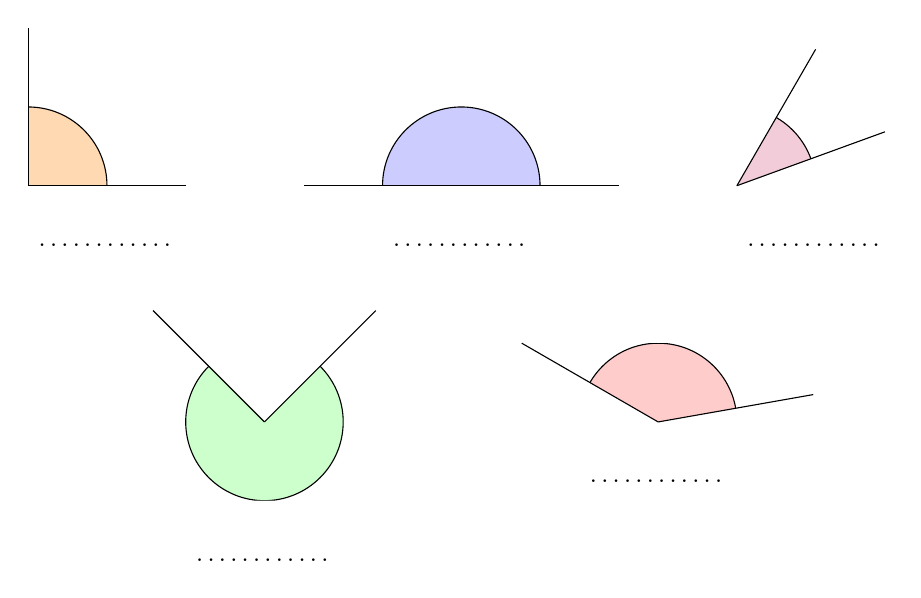
\begin{tikzpicture}[scale=1,font=\small]
\usetikzlibrary{calc}

\begin{scope}[xshift=-1.5cm]
\pgfmathsetmacro{\aalpha}{0};
\pgfmathsetmacro{\abeta}{90};
\coordinate (o) at (0,0);
\begin{scope}
\clip (o) rectangle (1.5,1.5);
\draw[fill=orange!30] (o) circle (1cm);
\end{scope}
\draw (o) -- +({\aalpha}:2);
\draw (o) -- +({\abeta}:2);
\node at (1,-.75) {\ldots\ldots\ldots\ldots};
\end{scope}

\begin{scope}[xshift=4cm]
\pgfmathsetmacro{\aalpha}{0};
\pgfmathsetmacro{\abeta}{180};
\coordinate (o) at (0,0);
\begin{scope}
\clip (-1.5,0) rectangle (1.5,1.5);
\draw[fill=blue!20] (o) circle (1cm);
\end{scope}
\draw (o) -- +({\aalpha}:2);
\draw (o) -- +({\abeta}:2);
\node at (0,-.75) {\ldots\ldots\ldots\ldots};
\end{scope}

\begin{scope}[xshift=7.5cm]
\pgfmathsetmacro{\aalpha}{20};
\pgfmathsetmacro{\abeta}{60};
\coordinate (o) at (0,0);
\begin{scope}
\clip (o) -- ({\aalpha}:1.5) -- ({\abeta}:1.5) -- cycle;
\draw[fill=purple!20] (o) circle (1cm);
\end{scope}
\draw (o) -- +({\aalpha}:2);
\draw (o) -- +({\abeta}:2);
\node at (1,-.75) {\ldots\ldots\ldots\ldots};
\end{scope}

\begin{scope}[xshift=1.5cm, yshift=-3cm]
\pgfmathsetmacro{\aalpha}{135};
\pgfmathsetmacro{\abeta}{405};
\coordinate (o) at (0,0);
\begin{scope}
\clip (o) -- ({\aalpha}:1.5) -- (-1.5,0) -- (-1.5,-1) -- (1.5,-1) -- (1.5,0) -- ({\abeta}:1.5) -- cycle;
\draw[fill=green!20] (o) circle (1cm);
\end{scope}
\draw (o) -- +({\aalpha}:2);
\draw (o) -- +({\abeta}:2);
\node at (0,-1.75) {\ldots\ldots\ldots\ldots};
\end{scope}

\begin{scope}[xshift=6.5cm, yshift=-3cm]
\pgfmathsetmacro{\aalpha}{10};
\pgfmathsetmacro{\abeta}{150};
\coordinate (o) at (0,0);
\begin{scope}
\clip (o) -- ({\aalpha}:1.5) -- (1.5,1) -- (-1.5,1) -- ({\abeta}:1.5) -- cycle;
\draw[fill=red!20] (o) circle (1cm);
\end{scope}
\draw (o) -- +({\aalpha}:2);
\draw (o) -- +({\abeta}:2);
\node at (0,-0.75) {\ldots\ldots\ldots\ldots};
\end{scope}

\end{tikzpicture}

\end{inaccessibleblock}
\end{center}


\end{esercizio}

% 
% \begin{inaccessibleblock}[Figura: TODO]
%  \begin{figure}[htb]
%  \centering% Copyright (c) 2015 Daniele Masini - d.masini.it@gmail.com

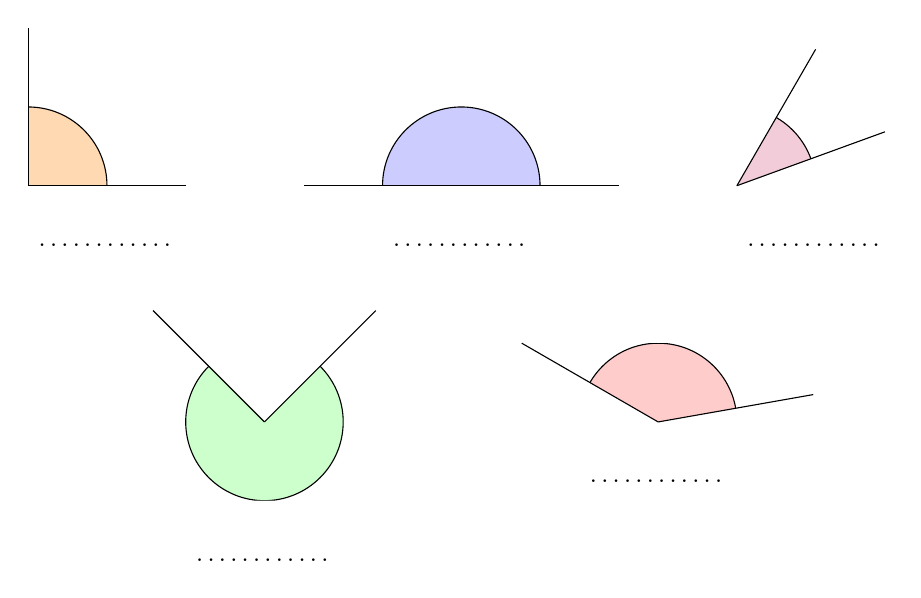
\begin{tikzpicture}[scale=1,font=\small]
\usetikzlibrary{calc}

\begin{scope}[xshift=-1.5cm]
\pgfmathsetmacro{\aalpha}{0};
\pgfmathsetmacro{\abeta}{90};
\coordinate (o) at (0,0);
\begin{scope}
\clip (o) rectangle (1.5,1.5);
\draw[fill=orange!30] (o) circle (1cm);
\end{scope}
\draw (o) -- +({\aalpha}:2);
\draw (o) -- +({\abeta}:2);
\node at (1,-.75) {\ldots\ldots\ldots\ldots};
\end{scope}

\begin{scope}[xshift=4cm]
\pgfmathsetmacro{\aalpha}{0};
\pgfmathsetmacro{\abeta}{180};
\coordinate (o) at (0,0);
\begin{scope}
\clip (-1.5,0) rectangle (1.5,1.5);
\draw[fill=blue!20] (o) circle (1cm);
\end{scope}
\draw (o) -- +({\aalpha}:2);
\draw (o) -- +({\abeta}:2);
\node at (0,-.75) {\ldots\ldots\ldots\ldots};
\end{scope}

\begin{scope}[xshift=7.5cm]
\pgfmathsetmacro{\aalpha}{20};
\pgfmathsetmacro{\abeta}{60};
\coordinate (o) at (0,0);
\begin{scope}
\clip (o) -- ({\aalpha}:1.5) -- ({\abeta}:1.5) -- cycle;
\draw[fill=purple!20] (o) circle (1cm);
\end{scope}
\draw (o) -- +({\aalpha}:2);
\draw (o) -- +({\abeta}:2);
\node at (1,-.75) {\ldots\ldots\ldots\ldots};
\end{scope}

\begin{scope}[xshift=1.5cm, yshift=-3cm]
\pgfmathsetmacro{\aalpha}{135};
\pgfmathsetmacro{\abeta}{405};
\coordinate (o) at (0,0);
\begin{scope}
\clip (o) -- ({\aalpha}:1.5) -- (-1.5,0) -- (-1.5,-1) -- (1.5,-1) -- (1.5,0) -- ({\abeta}:1.5) -- cycle;
\draw[fill=green!20] (o) circle (1cm);
\end{scope}
\draw (o) -- +({\aalpha}:2);
\draw (o) -- +({\abeta}:2);
\node at (0,-1.75) {\ldots\ldots\ldots\ldots};
\end{scope}

\begin{scope}[xshift=6.5cm, yshift=-3cm]
\pgfmathsetmacro{\aalpha}{10};
\pgfmathsetmacro{\abeta}{150};
\coordinate (o) at (0,0);
\begin{scope}
\clip (o) -- ({\aalpha}:1.5) -- (1.5,1) -- (-1.5,1) -- ({\abeta}:1.5) -- cycle;
\draw[fill=red!20] (o) circle (1cm);
\end{scope}
\draw (o) -- +({\aalpha}:2);
\draw (o) -- +({\abeta}:2);
\node at (0,-0.75) {\ldots\ldots\ldots\ldots};
\end{scope}

\end{tikzpicture}

%  \caption{Esercizio~\ref{ese:1.76}}\label{fig:ese1.76}
% \end{figure}
% \end{inaccessibleblock}

\begin{esercizio}
\label{ese:1.77}
Per ognuna delle seguenti affermazioni indica se è vera oppure falsa
\vspace{-6pt}
\begin{enumeratea}
\item Sommando due angoli acuti si ottiene sempre un angolo acuto
\hfill\boxV\quad\boxF
\item Sommando due angoli piatti si ottiene un angolo giro
\hfill\boxV\quad\boxF
\item Sommando un angolo acuto e uno retto si ottiene un angolo ottuso
\hfill\boxV\quad\boxF
\item Sommando due angoli retti si ottiene un angolo giro
\hfill\boxV\quad\boxF
\item Sommando un angolo piatto e un angolo acuto si ottiene un 
angolo concavo
\hfill\boxV\quad\boxF
\item Sommando due angoli convessi si ottiene sempre un angolo convesso
\hfill\boxV\quad\boxF
\item Sommando un angolo retto e un angolo piatto si ottiene un 
angolo giro
\hfill\boxV\quad\boxF
\end{enumeratea}
\hfill[a)~F,\quad b)~V,\quad c)~V,\quad d)~V,\quad e)~V,\quad f)~F,\quad 
g)~F]
\end{esercizio}

\begin{esercizio}
\label{ese:1.78}
Individua l'angolo
\vspace{-6pt}
\begin{enumeratea}
\item La differenza tra un angolo piatto è un angolo retto è un 
angolo \ldots\ldots\ldots\ldots\ldots\ldots{}
\item La differenza tra un angolo giro e un angolo piatto è un angolo 
\ldots\ldots\ldots\ldots\ldots\ldots{}
\item La differenza tra un angolo acuto e un angolo retto è un angolo 
\ldots\ldots\ldots\ldots\ldots\ldots{}
\item La differenza tra un angolo giro e un angolo piatto è un angolo 
\ldots\ldots\ldots\ldots\ldots\ldots{}
\item Il doppio di un angolo piatto è un angolo 
\ldots\ldots\ldots\ldots\ldots\ldots{}
\item Il doppio di un angolo retto è un angolo 
\ldots\ldots\ldots\ldots\ldots\ldots{}
\end{enumeratea}
\end{esercizio}
	
\begin{esercizio}
\label{ese:1.79}
Spiega perché se due angoli sono complementari i loro doppi sono 
supplementari.
\end{esercizio}

\begin{esercizio}
\label{ese:1.80}
Verifica, aiutandoti con un disegno, che se \(\widehat{A}\cong 
\widehat{B}\) e \(\widehat{C}<\widehat{D}\) allora 
\(\widehat{A}+\widehat{C}<\widehat{B}+\widehat{D}\).
\end{esercizio}

\begin{esercizio}
\label{ese:1.81}
Un angolo \(\alpha\) è retto e un angolo \(\beta\) è la sesta parte di un 
angolo piatto. A quale frazione di angolo retto corrisponde la somma 
\(\alpha + \beta\)?
\hfill[\(\frac{4}{3}\)]
\end{esercizio}

\begin{esercizio}
\label{ese:1.82}
Dati quattro segmenti \(AB>BC>CD>DE\). Verifica, aiutandoti con dei 
disegni, che:
\vspace{-6pt}
\begin{multicols}{2}
\begin{enumeratea}
\item \(AB-CD > BC-CD\);
\item \(AB+DE > BC+CD\).
\end{enumeratea}
\end{multicols}
\end{esercizio}

\begin{esercizio}
\label{ese:1.83}
Disegna due angoli consecutivi \(\alpha\) e \(\beta\), disegna l'angolo 
\(\gamma\) adiacente ad \(\alpha\) non contenente \(\beta\) e l'angolo 
\(\delta\) adiacente a \(\beta\) non contenente \(\alpha\). Gli angoli 
\(\gamma + \delta\) e \(\alpha+\beta\) sono:
\vspace{-6pt}
\begin{multicols}{2}
\begin{enumeratea}
\item complementari;
\item supplementari;
\item opposti al vertice;
\item esplementari.
\end{enumeratea}
\end{multicols}
\vspace{-18pt}
\hfill[b]
\end{esercizio}

\begin{multicols}{2}
 
\begin{esercizio}
\label{ese:1.84}
Su una semiretta di origine \(A\) segna il segmento \(AB\), il segmento 
\(BC\cong 3\cdot AB\) e il segmento \(CD\cong AB\), i punti sono 
consecutivi secondo l'ordine alfabetico. Secondo quale numero 
frazionario \(AD\) è multiplo di \(BC\)?
\hfill[\(\frac{5}{3}\)]
\end{esercizio}

\begin{esercizio}
\label{ese:1.87}
Su una retta, i punti \(A\), \(B\), \(C\), \(D\) si susseguono secondo 
l'ordine alfabetico. Se \(AB\) è congruente a \(CD\) i punti medi di \(BC\) 
e \(AD\) coincidono? Spiega perché?
\hfill[\dots]
\end{esercizio}

\begin{esercizio}
\label{ese:1.89}
Siano \(AB\) e \(CD\) due segmenti congruenti disposti su una retta \(r\), 
non aventi alcun punto in comune e in modo che \(AB\) preceda \(CD\). 
Dimostra che il punto medio di \(BC\) è anche punto medio di \(AD\).
\hfill[\dots]
\end{esercizio}

\begin{esercizio}
\label{ese:1.92}
Siano \(AB\) e \(BC\) due segmenti adiacenti non necessariamente 
congruenti, sia \(M\) il punto medio di \(AC\) ed \(N\) il punto medio di 
\(BC\), dimostra che \(MN\cong \frac{1}{2}\cdot AB\).
\hfill[\dots]
\end{esercizio}

\begin{esercizio}
\label{ese:1.95}
In un piano gli angoli \(A\widehat{O}C\) e \(C\widehat{O}D\) sono 
adiacenti. Sia \(OF\) la bisettrice di \(A\widehat{O}C\) e \(OE\) la 
bisettrice di \(C\widehat{O}D\). Spiega perché \(F\widehat{O}E\) è retto.
\hfill[\dots]
\end{esercizio}

% \begingroup
% \hypersetup{linkcolor=black}
% \subsubsection*{\ref{sect:misura} - \nameref{sect:misura}}
% \endgroup

\end{multicols}

\begingroup
\hypersetup{linkcolor=black}
\subsubsection*{\ref{sect:poligoni} - \nameref{sect:poligoni}}
\endgroup

\begin{esercizio}
\label{ese:1.125}
Quante diagonali ha un triangolo?
% \begin{multicols}{4}
% \begin{enumeratea}
% \item nessuna;
% \item 1;
% \item 2;
% \item 3.
% \end{enumeratea}
% \end{multicols}
% \vspace{-2.3em}
% \hfill[a]
\end{esercizio}

\begin{esercizio}
\label{ese:1.126}
Quante diagonali puoi tracciare dal vertice di un poligono di 6 lati?
% \begin{multicols}{4}
% \begin{enumeratea}
% \item 6;
% \item 5;
% \item 4;
% \item 3.
% \end{enumeratea}
% \end{multicols}
% \vspace{-2.3em}
% \hfill[d]
\end{esercizio}

% % \newpage

\begin{esercizio}
\label{ese:1.127}
Traccia l'angolo esterno relativo agli angoli interni indicati con un 
arco nella figura.
\end{esercizio}
\begin{center}
 \begin{inaccessibleblock}[Figura: TODO]
 % Copyright (c) 2015 Daniele Masini - d.masini.it@gmail.com

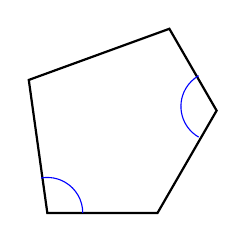
\begin{tikzpicture}[scale=1,font=\small]
\usetikzlibrary{calc}

\begin{scope}
\pgfmathsetmacro{\aalpha}{60};
\pgfmathsetmacro{\abeta}{120};
\pgfmathsetmacro{\agamma}{200};

\coordinate (o) at (0,0);

\draw[thick] (o) -- ++(0:1.4) -- ++({\aalpha}:1.5) -- ++({\abeta}:1.2) -- ++({\agamma}:1.9) -- cycle;

\draw[blue]
([shift=(0:.45)]o) arc [radius=.45, start angle={0}, end angle={360+\aalpha-\abeta-\agamma}]
++(0:1.7)
+([shift=({\aalpha+180}:.45)]{\aalpha}:1.05) arc [radius=.45, start angle={\aalpha+180}, end angle={\abeta}]
%++([shift=({\abeta+180}:.45)]{\abeta}:0.75) arc [radius=.45, start angle={\abeta+180}, end angle={\agamma}]
%++([shift=({\agamma+180}:.45)]{\agamma}:1.45) arc [radius=.45, start angle={\agamma+180}, end angle={540+\aalpha-\abeta-\agamma}]
;
\end{scope}

\end{tikzpicture}

\end{inaccessibleblock}
\end{center}



% \begin{inaccessibleblock}[Figura: TODO]
%  \begin{figure}[htb]
%  \centering% Copyright (c) 2015 Daniele Masini - d.masini.it@gmail.com

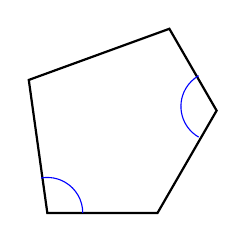
\begin{tikzpicture}[scale=1,font=\small]
\usetikzlibrary{calc}

\begin{scope}
\pgfmathsetmacro{\aalpha}{60};
\pgfmathsetmacro{\abeta}{120};
\pgfmathsetmacro{\agamma}{200};

\coordinate (o) at (0,0);

\draw[thick] (o) -- ++(0:1.4) -- ++({\aalpha}:1.5) -- ++({\abeta}:1.2) -- ++({\agamma}:1.9) -- cycle;

\draw[blue]
([shift=(0:.45)]o) arc [radius=.45, start angle={0}, end angle={360+\aalpha-\abeta-\agamma}]
++(0:1.7)
+([shift=({\aalpha+180}:.45)]{\aalpha}:1.05) arc [radius=.45, start angle={\aalpha+180}, end angle={\abeta}]
%++([shift=({\abeta+180}:.45)]{\abeta}:0.75) arc [radius=.45, start angle={\abeta+180}, end angle={\agamma}]
%++([shift=({\agamma+180}:.45)]{\agamma}:1.45) arc [radius=.45, start angle={\agamma+180}, end angle={540+\aalpha-\abeta-\agamma}]
;
\end{scope}

\end{tikzpicture}

%  \caption{Esercizio~\ref{ese:1.127}}\label{fig:ese1.127}
% \end{figure}
% \end{inaccessibleblock}

\begin{esercizio}
\label{ese:1.128}
Quali tra le seguenti figure geometriche sono sempre congruenti tra 
loro?
\begin{multicols}{2}
\begin{enumeratea}
\item Tutti i punti                \hfill \boxV\quad\boxF
\item Tutte le rette               \hfill \boxV\quad\boxF
\item Tutte le semirette           \hfill \boxV\quad\boxF
\item Tutti i semipiani            \hfill \boxV\quad\boxF
\item Tutti gli angoli             \hfill \boxV\quad\boxF
\item Tutti i poligoni convessi    \hfill \boxV\quad\boxF
\item Tutti i triangoli            \hfill \boxV\quad\boxF
\item Tutti i triangoli equilateri \hfill \boxV\quad\boxF
\item Tutti i quadrati             \hfill \boxV\quad\boxF
\end{enumeratea}
\end{multicols}
\hfill[a)~V,\quad b)~V,\quad c)~V,\quad d)~V,\quad e)~F,\quad f)~F,\quad 
g)~F,\quad h)~F,\quad i)~F]
\end{esercizio}

%\pagebreak

\begin{esercizio}[Prove invalsi 2006]
\label{ese:1.129}
Che cosa si definisce ``diagonale'' in un poligono convesso? Un 
segmento che
\begin{enumeratea}
\item congiunge due vertici non consecutivi del poligono;
\item congiunge due vertici qualsiasi del poligono;
\item congiunge i punti medi di due lati consecutivi del poligono;
\item divide il poligono in due parti congruenti.
\end{enumeratea}
\vspace{-2em}
\hfill[a]
\end{esercizio}

	
\begin{esercizio}[Prove invalsi 2006]
\label{ese:1.130}
Scegli tra le figure riportate nella figura~\ref{fig:ese1.130} quella 
in cui risulta vera l'uguaglianza \(\dfrac{AC}{CB}=\dfrac{3}{4}\).
\begin{center}
\begin{inaccessibleblock}[Figura: TODO]
 % Copyright (c) 2015 Daniele Masini - d.masini.it@gmail.com

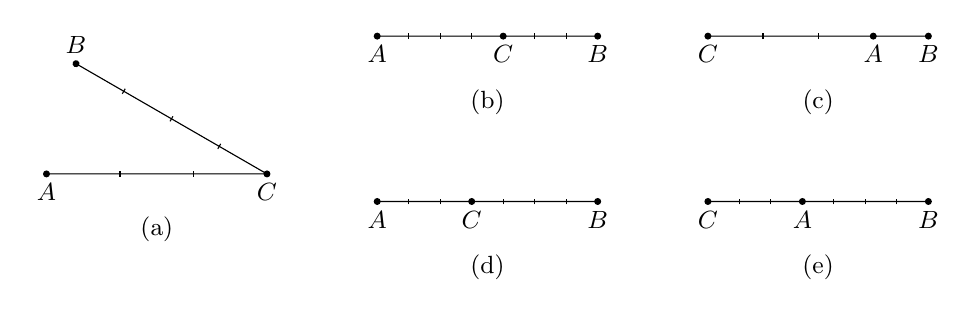
\begin{tikzpicture}[scale=.7,font=\small]
\usetikzlibrary{calc}

\begin{scope}[yshift=-2.5cm,rotate=150]
\coordinate (o) at (0,0);
\draw[fill] (o) -- (4,0) circle (1.5pt) node[above] {$B$};
\foreach \x in {1,2,3}
{
	\draw (\x,-1.5pt) -- (\x,1.5pt);
}
\end{scope}

\begin{scope}[yshift=-2.5cm,xshift=-4cm]
\coordinate (o) at (0,0);
\draw[fill] (o) circle (1.5pt) node[below] {$A$} -- (4,0) circle (1.5pt) node[below] {$C$};
\foreach \x in {1.333,2.666}
{
	\draw (\x,-1.5pt) -- (\x,1.5pt);
}
\node at (2,-1) {(a)};
\end{scope}

\begin{scope}[xshift=2cm]
\coordinate (o) at (0,0);
\draw[fill] (o) circle (1.5pt) node[below] {$A$} -- (4,0) circle (1.5pt) node[below] {$B$};
\foreach \x in {0.57142,1.142857,...,3.428572}
{
	\draw (\x,-1.5pt) -- (\x,1.5pt);
}
\draw[fill] (2.285714,0) circle (1.5pt) node[below] {$C$};
\node at (2,-1.2) {(b)};
\end{scope}

\begin{scope}[xshift=8cm]
\coordinate (o) at (0,0);
\draw[fill] (o) circle (1.5pt) node[below] {$C$} -- (4,0) circle (1.5pt) node[below] {$B$};
\foreach \x in {1,2}
{
	\draw (\x,-1.5pt) -- (\x,1.5pt);
}
\draw[fill] (3,0) circle (1.5pt) node[below] {$A$};
\node at (2,-1.2) {(c)};
\end{scope}

\begin{scope}[xshift=2cm, yshift=-3cm]
\coordinate (o) at (0,0);
\draw[fill] (o) circle (1.5pt) node[below] {$A$} -- (4,0) circle (1.5pt) node[below] {$B$};
\foreach \x in {0.57142,1.142857,...,3.428572}
{
	\draw (\x,-1.5pt) -- (\x,1.5pt);
}
\draw[fill] (1.714285,0) circle (1.5pt) node[below] {$C$};
\node at (2,-1.2) {(d)};
\end{scope}

\begin{scope}[xshift=8cm, yshift=-3cm]
\coordinate (o) at (0,0);
\draw[fill] (o) circle (1.5pt) node[below] {$C$} -- (4,0) circle (1.5pt) node[below] {$B$};
\foreach \x in {0.57142,1.142857,...,3.428572}
{
	\draw (\x,-1.5pt) -- (\x,1.5pt);
}
\draw[fill] (1.714285,0) circle (1.5pt) node[below] {$A$};
\node at (2,-1.2) {(e)};
\end{scope}

\end{tikzpicture}

\end{inaccessibleblock}
\end{center}
\vspace{-2.3em}
\hfill[d]
\end{esercizio}


% \begin{inaccessibleblock}[Figura: TODO]
%  \begin{figure}[htb]
%  \centering% Copyright (c) 2015 Daniele Masini - d.masini.it@gmail.com

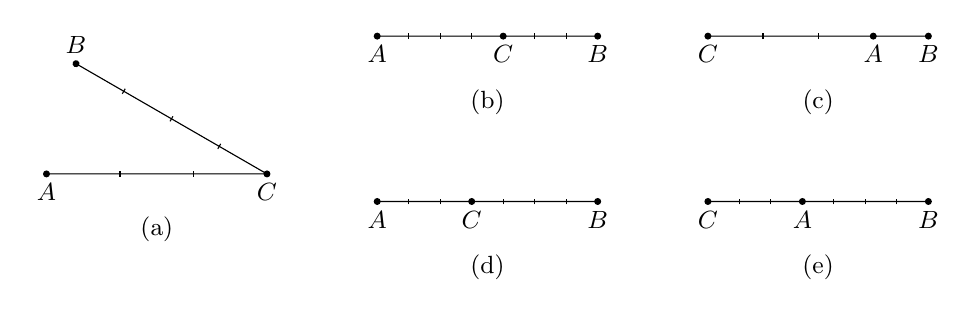
\begin{tikzpicture}[scale=.7,font=\small]
\usetikzlibrary{calc}

\begin{scope}[yshift=-2.5cm,rotate=150]
\coordinate (o) at (0,0);
\draw[fill] (o) -- (4,0) circle (1.5pt) node[above] {$B$};
\foreach \x in {1,2,3}
{
	\draw (\x,-1.5pt) -- (\x,1.5pt);
}
\end{scope}

\begin{scope}[yshift=-2.5cm,xshift=-4cm]
\coordinate (o) at (0,0);
\draw[fill] (o) circle (1.5pt) node[below] {$A$} -- (4,0) circle (1.5pt) node[below] {$C$};
\foreach \x in {1.333,2.666}
{
	\draw (\x,-1.5pt) -- (\x,1.5pt);
}
\node at (2,-1) {(a)};
\end{scope}

\begin{scope}[xshift=2cm]
\coordinate (o) at (0,0);
\draw[fill] (o) circle (1.5pt) node[below] {$A$} -- (4,0) circle (1.5pt) node[below] {$B$};
\foreach \x in {0.57142,1.142857,...,3.428572}
{
	\draw (\x,-1.5pt) -- (\x,1.5pt);
}
\draw[fill] (2.285714,0) circle (1.5pt) node[below] {$C$};
\node at (2,-1.2) {(b)};
\end{scope}

\begin{scope}[xshift=8cm]
\coordinate (o) at (0,0);
\draw[fill] (o) circle (1.5pt) node[below] {$C$} -- (4,0) circle (1.5pt) node[below] {$B$};
\foreach \x in {1,2}
{
	\draw (\x,-1.5pt) -- (\x,1.5pt);
}
\draw[fill] (3,0) circle (1.5pt) node[below] {$A$};
\node at (2,-1.2) {(c)};
\end{scope}

\begin{scope}[xshift=2cm, yshift=-3cm]
\coordinate (o) at (0,0);
\draw[fill] (o) circle (1.5pt) node[below] {$A$} -- (4,0) circle (1.5pt) node[below] {$B$};
\foreach \x in {0.57142,1.142857,...,3.428572}
{
	\draw (\x,-1.5pt) -- (\x,1.5pt);
}
\draw[fill] (1.714285,0) circle (1.5pt) node[below] {$C$};
\node at (2,-1.2) {(d)};
\end{scope}

\begin{scope}[xshift=8cm, yshift=-3cm]
\coordinate (o) at (0,0);
\draw[fill] (o) circle (1.5pt) node[below] {$C$} -- (4,0) circle (1.5pt) node[below] {$B$};
\foreach \x in {0.57142,1.142857,...,3.428572}
{
	\draw (\x,-1.5pt) -- (\x,1.5pt);
}
\draw[fill] (1.714285,0) circle (1.5pt) node[below] {$A$};
\node at (2,-1.2) {(e)};
\end{scope}

\end{tikzpicture}

%  \caption{Esercizio~\ref{ese:1.130}}\label{fig:ese1.130}
% \end{figure}
% \end{inaccessibleblock}

\begin{esercizio}[Prove invalsi 2005]
\label{ese:1.131}
Due segmenti misurano 5~dm e 30~cm rispettivamente. Qual è il 
rapporto fra la lunghezza del secondo segmento e quella del primo?
\begin{multicols}{4}
\begin{enumeratea}
\item 6;
\item \(5/3\);
\item \(3/5\);
\item \(1/6\).
\end{enumeratea}
\end{multicols}
\vspace{-2.3em}
\hfill[c]
\end{esercizio}

\begin{esercizio}[Prove invalsi 2005]
\label{ese:1.132}
I punti \(A\), \(B\) e \(C\) sono allineati come nella 
figura. Se l'angolo \(A\widehat{B}E\) misura 
\(54\grado\) e \(BD\) è la bisettrice dell'angolo \(E\widehat{B}C\), quanto 
misura l'angolo \(D\widehat{B}C\)?

\begin{minipage}{.39 \textwidth}
\begin{center}
\begin{inaccessibleblock}[Retta CBA con due semirette BD e BE nello stesso 
semipiano.]
 % Copyright (c) 2015 Daniele Masini - d.masini.it@gmail.com

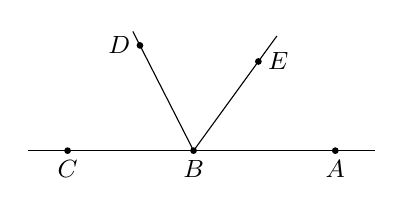
\begin{tikzpicture}[scale=1,font=\small]
\usetikzlibrary{calc}

\begin{scope}
\pgfmathsetmacro{\aalpha}{0};
\pgfmathsetmacro{\abeta}{54};
\pgfmathsetmacro{\agamma}{117};
\pgfmathsetmacro{\adelta}{180};

\draw (0,0) coordinate (b) node[below] {$B$} -- +({\aalpha}:2.3);
\draw[fill] (b) circle (1pt);
\draw[fill] +({\aalpha}:1.8) circle (1pt) node[below] {$A$};
\draw (b) -- +({\abeta}:1.8);
\draw[fill] +({\abeta}:1.4) circle (1pt) node[right] {$E$};
\draw (b) -- +({\agamma}:1.7);
\draw[fill] +({\agamma}:1.5) circle (1pt) node[left] {$D$};
\draw (b) -- +({\adelta}:2.1);
\draw[fill] +({\adelta}:1.6) circle (1pt) node[below] {$C$};
\end{scope}

\end{tikzpicture}

\end{inaccessibleblock}
\end{center}
\end{minipage}
\hfill
\begin{minipage}{.55 \textwidth}
\begin{multicols}{2}
\begin{enumeratea}
\item \(26\grado\)
\item \(36\grado\)
\item \(54\grado\)
\item \(63\grado\)
\end{enumeratea}
\end{multicols}
\vspace{-2.3em}
\hfill[d]
\end{minipage}

\end{esercizio}

% \begin{inaccessibleblock}[Figura: TODO]
%  \begin{figure}[htb]
%  \centering% Copyright (c) 2015 Daniele Masini - d.masini.it@gmail.com

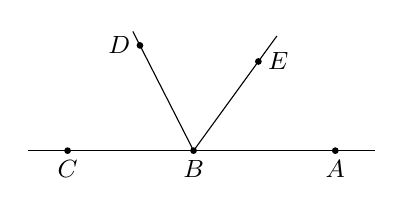
\begin{tikzpicture}[scale=1,font=\small]
\usetikzlibrary{calc}

\begin{scope}
\pgfmathsetmacro{\aalpha}{0};
\pgfmathsetmacro{\abeta}{54};
\pgfmathsetmacro{\agamma}{117};
\pgfmathsetmacro{\adelta}{180};

\draw (0,0) coordinate (b) node[below] {$B$} -- +({\aalpha}:2.3);
\draw[fill] (b) circle (1pt);
\draw[fill] +({\aalpha}:1.8) circle (1pt) node[below] {$A$};
\draw (b) -- +({\abeta}:1.8);
\draw[fill] +({\abeta}:1.4) circle (1pt) node[right] {$E$};
\draw (b) -- +({\agamma}:1.7);
\draw[fill] +({\agamma}:1.5) circle (1pt) node[left] {$D$};
\draw (b) -- +({\adelta}:2.1);
\draw[fill] +({\adelta}:1.6) circle (1pt) node[below] {$C$};
\end{scope}

\end{tikzpicture}

%  \caption{Esercizio~\ref{ese:1.132}}\label{fig:ese1.132}
% \end{figure}
% \end{inaccessibleblock}

%\pagebreak

\begin{esercizio}[Prove invalsi 2005]
\label{ese:1.133}
Un poligono è regolare se tutti i suoi lati sono uguali e tutti i 
suoi angoli sono uguali. Un poligono non è regolare se e solamente se 
\ldots
\begin{enumeratea}
\item tutti i suoi lati e tutti i suoi angoli sono disuguali;
\item tutti i suoi lati o tutti i suoi angoli sono disuguali;
\item almeno due dei suoi lati e almeno due dei suoi angoli sono tra 
loro disuguali;
\item almeno due dei suoi lati o almeno due dei suoi angoli sono tra 
loro disuguali.
\end{enumeratea}
\vspace{-2.3em}
\hfill[d]
\end{esercizio}
